\documentclass[../../main]{subfiles}

\begin{document}
\chapter{ヒルベルト空間}
\label{chapter:hilbert_space}

\begin{lead}
  \cref{chapter:hilbert_space}では,数ベクトルに対する議論を関数に対する議論へと拡張する.
  この拡張によって,連続時間の対象についてもベクトル空間の考え方が適用可能になる.
\end{lead}

\section{イントロダクション}

\begin{figure}[htbp]
  \centering
  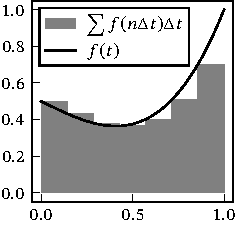
\includegraphics{figures/riemann_sum.pdf}
  \caption{\(f(t)\)と\(\sum f(n\increment t)\increment t\)の比較.}
\end{figure}

\[
  \sum_{n=0}^{N-1}x(n\increment t)\conj*{y(n\increment t)}\increment t \to \int_0^1x(t)\conj*{y(t)}\intd{t}\quad(N\to\infty)
\]

\section{無限次元のベクトル空間}

\subsection{距離空間}

\begin{definition}{距離}{metric}\index{きょり@距離}
  \(S\)を集合とする.\(d\)が\(S\)上の\termdef{距離}(metric)であるとは,
  任意の\(x,y,z\in S\)に対して,\(d\)が以下の条件を満たすことをいう.
  \begin{enumerate}
    \item \(d(x,y)\geq 0\),\([d(x,y)=0\iff x=y]\)
    \item \(d(x,y)=d(y,x)\)
    \item \(d(x,y)+d(y,z)\geq d(x,z)\)
  \end{enumerate}
\end{definition}

集合と距離の組\((S,d)\)を\termdef{距離空間}\index{きょりくうかん@距離空間}(metric space)という.

\begin{example}
  \label{example:metric_space}
  \(S=\numset{C}\),\(d(z,w)=\abs{z-w}\)とすると,\((S,d)\)は距離空間になる.
\end{example}

\begin{example}[離散距離]
  \label{example:discrete_metric}
  集合\(S\)は空でないとする.また,各\(x,y\in S\)に対して,\(x=y\)のとき\(d(x,y)=0\),\(x\neq y\)のとき\(d(x,y)=1\)とする.
  このとき\(d\)は\(S\)上の距離になる.距離\(d\)を\termdef{離散距離}\index{りさんきょり@離散距離}(discrete metric),
  距離空間\((S,d)\)を\termdef{離散空間}\index{りさんくうかん@離散空間}(discrete space)という.
\end{example}

\cref{definition:metric}のように抽象的な形で距離を定義する利点の1つは,\(\numset{K}^n\)以外の集合に対しても,点列の極限を定義できることである.

\begin{definition}{点列の収束}{sequence_converge}\index{しゅうそくてんれつの@収束,点列の}
  \((S,d)\)を距離空間とする.\(S\)上の点列\(\seq{x_n}_{n\in\numset{N}}\)が\(\alpha\in S\)に\termdef{収束する}(converge)とは,
  任意の\(\varepsilon>0\)に対し,\(N\in\numset{N}\)が存在して\(n>N\implies d(x_n,\alpha)<\varepsilon\)を満たすことをいう.
  このことを次のように表す.
  \[
    x_n\to\alpha\quad(n\to\infty)
  \]
\end{definition}

\begin{note}
  次の命題が成り立つことに注意.
  \[
    x_n \to \alpha\quad(n\to\infty)
    \iff\lim_{n\to\infty}d(x_n,\alpha) = 0
  \]
\end{note}

\(\seq{x_n}_{n\in\numset{N}}\)が\(\alpha\)に収束するとき,\(\alpha\)を\(\seq{x_n}_{n\in\numset{N}}\)の\termdef{極限点}\index{きょくげんてん@極限点}(limit point)という.
\cref{definition:sequence_converge}は要するに「\(N\)の値を十分に大きくとれば,点\(x_{N+1},x_{N+2},\dotsc\)が点\(\alpha\)から距離\(\varepsilon\)以上離れないようにできる」ことを意味する.

\begin{example}
  \label{example:complex_planes_convergence}
  \((S,d)\)を\cref{example:metric_space}の距離空間とする.\(S\)上の点列\(\seq{z_n}_{n\in\numset{N}}\)を\(z_n=(\sqrt{3}+\iuni)/(2n)\)で定義すると,
  \(\seq{z_n}_{n\in\numset{N}}\)は\cref{definition:sequence_converge}の意味で\(z_n\to 0\)(\(n\to\infty\))を満たす.
\end{example}

\begin{example}[一様収束]
  \label{example:uniform_converge}
  閉区間\(I\)は有界とする.連続関数\(f\colon I\to\numset{R}\)の全体集合を\(\cont{0}(I)\)とおくと,\(d(f,g)=\max\Set{\abs{f(x)-g(x)}\given x\in I}\)は\(\cont{0}(I)\)上の距離になる.
  \(\cont{0}(I)\)上の関数列\(\seq{f_n}_{n\in\numset{N}}\)が\cref{definition:sequence_converge}の意味で\(f\in\cont{0}(I)\)に収束するとき,
  \(\seq{f_n}_{n\in\numset{N}}\)は\(f\)に\termdef{一様収束する}\index{いちようしゅうそく@一様収束}(converge uniformly)という.

  たとえば\(I=[0,1]\),\(f_n(x)=(1/n)\abs{\sin(n\krez x)}\)のとき,\(\seq{f_n}_{n\in\numset{N}}\)は定数関数\(\phi(x)=0\)に一様収束する.
  実際\(d(f_n,\phi)=\max\Set{\abs{f_n(x)}\given x\in I}=1/n\)なので,\(n\)の値を十分大きくとれば\(d(f_n,\phi)\)の値を限りなく小さくできる(\cref{figure:uniform_converge}).
\end{example}

\begin{figure}[htbp]
  \begin{minipage}{0.5\linewidth}
    \centering
    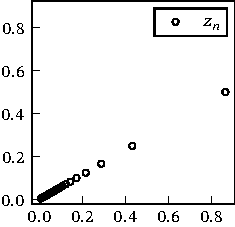
\includegraphics{figures/complex_convergence.pdf}
    \caption{\(z_n\to 0\)(\(n\to\infty\))の様子.}
    \label{figure:sequence_converge}
  \end{minipage}%
  \begin{minipage}{0.5\linewidth}
    \centering
    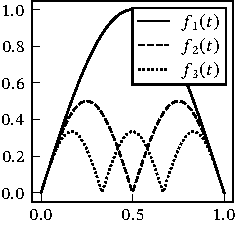
\includegraphics{figures/func_convergence.pdf}
    \caption{\(f_n\to\phi\)(\(n\to\infty\))の様子.}
    \label{figure:uniform_converge}
  \end{minipage}
\end{figure}

\begin{note}
  \cref{example:complex_planes_convergence}において\(\abs{z_n}=1/n\)であるから,\(d(f_n,\phi)=\abs{z_n}\)である.
  よって,\cref{figure:sequence_converge}は(\(z_n\)を\(f_n\)に書き換えれば)\(f_n\to\phi\)(\(n\to\infty\))の様子を描いた図とも考えられる.
  このように,関数などの一見「点」とは思えないような対象を点とみなして考察するのは,しばしば理解の助けになる.
\end{note}

\begin{proposition}{}{limit_uniqueness}
  極限点は存在すれば一意である.すなわち,距離空間\((S,d)\)上の点列\(\seq{x_n}_{n\in\numset{N}}\)が\(\alpha,\beta\in S\)に収束するなら,\(\alpha=\beta\)である.
\end{proposition}

\begin{proof}
  \(0\leq d(\alpha,\beta)\leq d(\alpha,x_n)+d(x_n,\beta)=d(x_n,\alpha)+d(x_n,\beta)\)なので,\(d(x_n,\alpha)\to 0\),\(d(x_n,\beta)\to 0\)(\(n\to\infty\))なら\(d(\alpha,\beta)=0\),\(\alpha=\beta\)である.
\end{proof}

\cref{proposition:limit_uniqueness}から,各収束列\(\seq{x_n}_{n\in\numset{N}}\)に対して,その極限点は一意に定まる.そのため,以降は収束列\(\seq{x_n}_{n\in\numset{N}}\)の極限点を
\[
  \lim_{n\to\infty}x_n
\]
と書く.

\begin{definition}{閉包・閉集合・稠密}{closure}\index{へいほう@閉包}\index{へいしゅうごう@閉集合}\index{ちゅうみつ@稠密}\index{cl@\(\clsr S\)}
  \((S,d)\)を距離空間,\(A\)を\(S\)の部分集合とする.
  \begin{enumerate}
    \item \(A\)上の収束列すべての極限点からなる集合を\(A\)の\termdef{閉包}(closure)といい,\(\clsr A\)と書く\footnotemark .
    \item \(A=\clsr A\)であるとき,\(A\)は\termdef{閉集合}(closed set)であるという.
    \item 集合\(B\subset A\)が\(\clsr B=A\)を満たすとき,\(B\)は\(A\)において\termdef{\ltjruby{稠密}{ちゆうみつ}}(dense)であるという.
  \end{enumerate}
\end{definition}

\footnotetext{本書では閉包を\(\clsr A\),補集合を\(\scomp{A}\)\index{c@\(\scomp{S}\)}で表す.}

\begin{example}
  \(\clsr\ocival{0}{1}=\ccival{0}{1}\),\(\clsr\numset{Q}=\numset{R}\)である.
\end{example}

\begin{definition}{コーシー列}{cauchy_sequence}\index{こーしーれつ@コーシー列}
  \((S,d)\)を距離空間とする.\(S\)上の点列\(\seq{x_n}_{n\in\numset{N}}\)が\termdef{コーシー列}(Cauchy sequence)であるとは,
  任意の\(\varepsilon>0\)に対し,\(N\in\numset{N}\)が存在して\(m,n>N\implies d(x_m,x_n)<\varepsilon\)を満たすことをいう.このことを次のように表す.
  \[
    d(x_m,x_n) \to 0\quad(m,n\to\infty),
    \quad\lim_{m,n\to\infty}d(x_m,x_n) = 0
  \]
\end{definition}

また,\(S\)上の任意のコーシー列が収束列でもあるとき,\((S,d)\)は\termdef{完備距離空間}\index{かんびきょりくうかん@完備距離空間}\index{きょりくうかん@距離空間!かんび@完備\texttwoemdash}(complete metric space)であるという.
一般に収束列はコーシー列でもあるから,完備距離空間において収束列とコーシー列は同値な概念である.

\begin{example}
  \(S=\numset{Q}\),\(d(x,y)=\abs{x-y}\)とすると,\((S,d)\)は距離空間になるが完備距離空間にはならない.
\end{example}

\subsection{ノルム空間}

\begin{definition}{ノルム}{norm}\index{のるむ@ノルム}\indexsymbol{\(\vnorm{\holder}\)}
  \(V\)を\(\numset{K}\)上のベクトル空間とする.\(\vnorm{\holder}\)が\(V\)の\termdef{ノルム}(norm)であるとは,
  任意の\(\lambda\in\numset{K}\),\(\vect{x},\vect{y}\in V\)に対して,\(\vnorm{\holder}\)が以下の条件を満たすことをいう.
  \begin{enumerate}
    \item \(\vnorm{\vect{x}}\geq 0\),\([\vnorm{\vect{x}}=0\iff\vect{x}=\zvec]\)
    \item \(\vnorm{\lambda\vect{x}}=\abs{\lambda}\vnorm{\vect{x}}\)
    \item \(\vnorm{\vect{x}+\vect{y}}\leq\vnorm{\vect{x}}+\vnorm{\vect{y}}\)
  \end{enumerate}
\end{definition}

ノルムが備わっているベクトル空間のことを\termdef{ノルム空間}\index{のるむくうかん@ノルム空間}(normed space)という.
\(V\)がノルム空間であれば,\(d(\vect{x},\vect{y})=\vnorm{\vect{x}-\vect{y}}\)(\(\vect{x},\vect{y}\in V\))により\(V\)上の距離\(d\)が定義される.
\((V,d)\)が完備距離空間であるとき,\(V\)は\termdef{バナッハ空間}\index{ばなっはくうかん@バナッハ空間}(Banach space)であるという.

\begin{example}
  \(V\)が\(\numset{K}\)上の内積空間なら,\(V\)の内積\(\innerp{\holder}{\holder}\)から\(V\)のノルムを\(\vnorm{\vect{x}}=\sqrt{\innerp{\vect{x}}{\vect{x}}}\)で定義できる.
  つまり,内積空間はノルム空間でもある.
\end{example}

\begin{example}[\(\lebesgue{p}\)空間]
  複素数列\(\seq{x_n}_{n\in\numset{N}}\)に対して,\(\vnorm{\seq{x_n}_{n\in\numset{N}}}_{\lebesgue{p}}\in\ccival{0}{\infty}\)(\(p\geq 1\))を
  \[
    \vnorm{\seq{x_n}_{n\in\numset{N}}}_{\lebesgue{p}} = \pqty*{\sum_{n=1}^\infty\abs{x_n}^p}^{1/p}
  \]
  で定義する.\(\numset{C}^{\numset{N}}\)の部分空間\(\lebesgue{p}(\numset{N})\)を\(\lebesgue{p}(\numset{N})=\Set*{\seq{x_n}_{n\in\numset{N}}\given\vnorm{\seq{x_n}_{n\in\numset{N}}}_{\lebesgue{p}}<\infty}\)
  で定義すると,\(\vnorm{\holder}_{\lebesgue{p}}\)は\(\lebesgue{p}\)のノルムになり,しかも,\(\lebesgue{p}(\numset{N})\)はこのノルムについてバナッハ空間になる.
  バナッハ空間\(\lebesgue{p}(\numset{N})\)を\termdef{\(\lebesgue{p}\)空間}\index{lpkukan@\(\lebesgue{p}\)空間}(\(\lebesgue{p}\) space)という.
\end{example}

\begin{example}
  \cref{example:uniform_converge}の集合\(\cont{0}(I)\)は,ノルム\(\vnorm{f}_\infty=\max\Set{\abs{f(x)}\given x\in I}\)についてバナッハ空間になる.
  ただし,関数の和\(\phi=f+g\)とスカラー倍\(\psi=\lambda f\)はそれぞれ\(\phi(x)=f(x)+g(x)\),\(\psi(x)=\lambda\cdot(f(x))\)で定義する.
\end{example}

\section{ヒルベルト空間}

\begin{definition}{ヒルベルト空間}{hilbert_space}\index{ひるべるとくうかん@ヒルベルト空間}
  内積空間\(H\)が\termdef{ヒルベルト空間}(Hilbert space)であるとは,
  \(H\)の内積\(\innerp{\holder}{\holder}\)から定まるノルム\(\vnorm{\vect{x}}=\sqrt{\innerp{\vect{x}}{\vect{x}}}\)について,\(H\)がバナッハ空間であることをいう.
\end{definition}

もう少し定義をさかのぼると,ノルム空間\(H\)がバナッハ空間であるとは,距離\(d(\vect{x},\vect{y})=\vnorm{\vect{x}-\vect{y}}\)について\((H,d)\)が完備距離空間であることをいうのであった.
したがって,完備距離空間・ノルム空間・バナッハ空間・内積空間が有する性質はすべて,ヒルベルト空間にも引き継がれる.

\begin{note}
  以下に述べる命題は,内積空間であればすべて成立する.内積空間がヒルベルト空間であるための条件「完備性」は,条件を満たす点列に対して,極限点の存在を保証するものである.
  そのため,ヒルベルト空間でないと成立しない定理は,存在を主張する定理であることが多い.
  本書においても,存在定理である\cref{theorem:convex_projection_theorem}で初めて,完備性が本質的に効いてくる.
\end{note}

\begin{theorem}{中線定理}{median_theorem}\index{ちゅうせんていり@中線定理}
  \(V\)を内積空間とするとき,任意の\(\vect{x},\vect{y}\in V\)に対して\(\vnorm{\vect{x}+\vect{y}}^2+\vnorm{\vect{x}-\vect{y}}^2=2(\vnorm{\vect{x}}^2+\vnorm{\vect{y}}^2)\)が成立する.
\end{theorem}

\begin{proof}
  実際\(\vnorm{\vect{x}+\vect{y}}^2+\vnorm{\vect{x}-\vect{y}}^2=(\vnorm{\vect{x}}^2+2\rpart\innerp{\vect{x}}{\vect{y}}+\vnorm{\vect{y}}^2)+(\vnorm{\vect{x}}^2-2\rpart\innerp{\vect{x}}{\vect{y}}+\vnorm{\vect{y}}^2)=2(\vnorm{\vect{x}}^2+\vnorm{\vect{y}}^2)\)である.
\end{proof}

\begin{theorem}{コーシー・シュワルツの不等式}{cauchy_schwarz}\index{こーしーしゅわるつのふとうしき@コーシー・シュワルツの不等式}
  \(V\)を内積空間とする.このとき,任意の\(\vect{a},\vect{b}\in V\)について\(\abs{\innerp{\vect{a}}{\vect{b}}}\leq\vnorm{\vect{a}}\vnorm{\vect{b}}\)が成立する.
  これを\termdef{コーシー・シュワルツの不等式}(Cauchy–Schwarz inequality)という.
\end{theorem}

\begin{proof}
  \(\vect{b}\neq\zvec\)のときについて示す.
  \(\lambda=\innerp{\vect{a}}{\vect{b}}/\vnorm{\vect{b}}^2\),\(\vect{a}_{\mathord{\perp}}=\vect{a}-\lambda\vect{b}\)とおくと,\(\innerp{\vect{a}_{\mathord{\perp}}}{\vect{b}}=0\)より
  \(
    \vnorm{\vect{a}_{\mathord{\perp}}}^2 = \innerp{\vect{a}_{\mathord{\perp}}}{\vect{a}_{\mathord{\perp}}}
    = \innerp{\vect{a}-\lambda\vect{b}}{\vect{a}_{\mathord{\perp}}}
    = \innerp{\vect{a}}{\vect{a}_{\mathord{\perp}}} - \lambda\innerp{\vect{b}}{\vect{a}_{\mathord{\perp}}}
    = \innerp{\vect{a}}{\vect{a}_{\mathord{\perp}}}
  \)
  である.よって
  \(
    \vnorm{\vect{a}_{\mathord{\perp}}}^2 = \innerp{\vect{a}}{\vect{a}-\lambda\vect{b}}
    = \vnorm{\vect{a}}^2-\conj{\lambda}\innerp{\vect{a}}{\vect{b}}
    = \vnorm{\vect{a}}^2-\abs{\innerp{\vect{a}}{\vect{b}}}^2/\vnorm{\vect{b}}^2
  \)
  だから,\((\vnorm{\vect{a}}\vnorm{\vect{b}})^2-\abs{\innerp{\vect{a}}{\vect{b}}}^2=(\vnorm{\vect{a}_{\mathord{\perp}}}\vnorm{\vect{b}})^2\geq 0\)である.
\end{proof}

\begin{proposition}{ノルムの連続性}{norm_continuous}
  \(V\)がノルム空間なら,\(V\)上の任意の収束列\(\seq{\vect{x}_n}\)について次式が成立する.
  \[
    \lim_{n\to\infty}\vnorm{\vect{x}_n} = \vnorm*{\lim_{n\to\infty}\vect{x}_n}
  \]
\end{proposition}

\begin{proof}
  \(\seq{\vect{x}_n}\)を\(V\)上の収束列とし,極限点を\(\vect{a}\)とおく.
  このとき\(\vnorm{\vect{x}_n}\leq\vnorm{\vect{x}_n-\vect{a}}+\vnorm{\vect{a}}\),\(\vnorm{\vect{a}}\leq\vnorm{\vect{a}-\vect{x}_n}+\vnorm{\vect{x}_n}\)なので
  \(\abs{\vnorm{\vect{x}_n}-\vnorm{\vect{a}}}\leq\vnorm{\vect{x}_n-\vect{a}}\to 0\)(\(n\to\infty\)),よって\(\vnorm{\vect{x}_n}\to\vnorm{\vect{a}}\)(\(n\to\infty\))である.
\end{proof}

\begin{proposition}{内積の連続性}{inner_products_continuous}
  \(V\)が内積空間なら,\(V\)上の任意の収束列\(\seq{\vect{x}_n}\),\(\seq{\vect{y}_n}\)について次式が成立する.
  \[
    \lim_{k\to\infty}\innerp{\vect{x}_k}{\vect{y}_k} = \innerp*{\lim_{m\to\infty}\vect{x}_m}{\lim_{n\to\infty}\vect{y}_n}
  \]
\end{proposition}

\begin{proof}
  \(\vect{x}_n\to\vect{a}\),\(\vect{y}_n\to\vect{b}\)(\(n\to\infty\))とする.
  \(\innerp{\vect{x}_n}{\vect{y}_n}=\innerp{\vect{x}_n-\vect{a}}{\vect{y}_n}+\innerp{\vect{a}}{\vect{y}_n-\vect{b}}+\innerp{\vect{a}}{\vect{b}}\)だから,
  \nameref{theorem:cauchy_schwarz}より\(\abs{\innerp{\vect{x}_n}{\vect{y}_n}-\innerp{\vect{a}}{\vect{b}}}\leq\abs{\innerp{\vect{x}_n-\vect{a}}{\vect{y}_n}}+\abs{\innerp{\vect{a}}{\vect{y}_n-\vect{b}}}\leq\vnorm{\vect{x}_n-\vect{a}}\vnorm{\vect{y}_n}+\vnorm{\vect{a}}\vnorm{\vect{y}_n-\vect{b}}\)である.
  \cref{proposition:norm_continuous}より\(\vnorm{\vect{x}_n-\vect{a}}\vnorm{\vect{y}_n}\to 0\vnorm{\vect{b}}\),\(\vnorm{\vect{y}_n-\vect{a}}\to 0\)(\(n\to\infty\))なので,\(\innerp{\vect{x}_n}{\vect{y}_n}\to\innerp{\vect{a}}{\vect{b}}\)(\(n\to\infty\))である.
\end{proof}

\section{直交射影}

\subsection{直交射影}

\begin{definition}{線分,凸集合}{convex_set}\index{せんぶん@線分}\index{とつしゅうごう@凸集合}
  \(V\)を\(\numset{K}\)上のベクトル空間とする.2点\(\vect{x},\vect{y}\in V\)に対して,集合\(\Set{(1-t)\vect{x}+t\vect{y}\given t\in\ccival{0}{1}}\)を
  \(\vect{x}\)と\(\vect{y}\)を結ぶ\termdef{線分}(line segment)という.
  また,集合\(S\subset V\)に属する任意の2点を結ぶ線分が\(S\)に含まれるとき,\(S\)は\termdef{凸集合}(convex set)であるという.
\end{definition}

\begin{figure}[htbp]
  \begin{minipage}{0.5\linewidth}
    \centering
    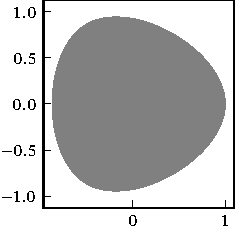
\includegraphics{figures/convex.pdf}
    \caption{\(\numset{R}^2\)の凸集合.}
  \end{minipage}%
  \begin{minipage}{0.5\linewidth}
    \centering
    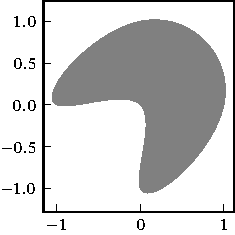
\includegraphics{figures/non_convex.pdf}
    \caption{\(\numset{R}^2\)の凸集合でない部分集合.}
  \end{minipage}
\end{figure}

\begin{theorem}{凸射影定理}{convex_projection_theorem}\index{とつしゃえいていり@凸射影定理}\index{しゃえいていり@射影定理!とつ@凸\texttwoemdash}
  \(H\)をヒルベルト空間とする.また,\(\vect{x}\in H\)かつ,集合\(C\subset H\)は空でない閉凸集合とする.
  このとき,\(\argmin_{\vect{y}\in C}\vnorm{\vect{x}-\vect{y}}\)はただ1つの元からなる集合である.
\end{theorem}

\begin{proof}
  まず,\(\argmin_{\vect{y}\in C}\vnorm{\vect{x}-\vect{y}}\)が空でないことを示す.\(\delta=\inf\Set{\vnorm{\vect{x}-\vect{y}}\given\vect{y}\in C}\)とおくと,
  集合\(A_n=\Set{\vect{y}\in C\given\vnorm{\vect{x}-\vect{y}}\leq\delta+1/n}\)(\(n=1,2,\dotsc\))は\(n\)の値によらず空でない.
  そこで,\(C\)上の点列\(\seq{\vect{a}_n}\)を各\(n\)に対して\(\vect{a}_n\in A_n\)となるようにとれる.
  \(0\leq\vnorm{\vect{x}-\vect{a}_n}-\delta\leq 1/n\to 0\)(\(n\to\infty\))なので,\(\seq{\vect{a}_n}\)がある点\(\vect{m}\)に収束すれば,\nameref{proposition:norm_continuous}より
  \(\vnorm{\vect{x}-\vect{m}}=\lim_{n\to\infty}\vnorm{\vect{x}-\vect{a}_n}=\delta\)である.さらに,\(C\)は閉集合だから\(\vect{m}\in C\),よって\(\vect{m}\in\argmin_{\vect{y}\in C}\vnorm{\vect{x}-\vect{y}}\)である.

  つまり,\(\seq{\vect{a}_n}\)の極限点\(\vect{m}\)が存在すること,すなわち,\(\seq{\vect{a}_n}\)がコーシー列であることを示せばよい.
  \(m,n\in\numset{N}\)を任意にとる.\nameref{theorem:median_theorem}より
  \begin{gather*}
    \vnorm{(\vect{a}_m-\vect{x})+(\vect{a}_n-\vect{x})}^2+\vnorm{\vect{a}_m-\vect{a}_n}^2 = 2(\vnorm{\vect{a}_m-\vect{x}}^2+\vnorm{\vect{a}_n-\vect{x}}^2), \\
    \vnorm{\vect{a}_m-\vect{a}_n}^2 = 2\vnorm{\vect{x}-\vect{a}_m}^2+2\vnorm{\vect{x}-\vect{a}_n}^2-4\vnorm*{\vect{x}-\frac{\vect{a}_m+\vect{a}_n}{2}}^2
  \end{gather*}
  である.\(\vect{a}_m\in A_m\),\(\vect{a}_n\in A_n\)かつ,\(C\)は凸集合だから\((\vect{a}_m+\vect{a}_n)/2\in C\)で
  \[
    \vnorm{\vect{a}_m-\vect{a}_n}^2 \leq 2\pqty*{\delta+\frac{1}{m}}^2+2\pqty*{\delta+\frac{1}{n}}^2-4\delta^2
    \to 0\quad(m,n\to\infty)
  \]
  である.よって\(\seq{\vect{a}_n}\)はコーシー列だから,\(\argmin_{\vect{y}\in C}\vnorm{\vect{x}-\vect{y}}\)は空でない.

  次に,\(\argmin_{\vect{y}\in C}\vnorm{\vect{x}-\vect{y}}\)の元は1つしかないことを示す.\(\vect{m}_1,\vect{m}_2\in\argmin_{\vect{y}\in C}\vnorm{\vect{x}-\vect{y}}\)とする.
  このとき\(\vnorm{\vect{x}-\vect{m}_1}=\vnorm{\vect{x}-\vect{m}_2}=\delta\),\((\vect{m}_1+\vect{m}_2)/2\in C\)なので\(\vnorm{\vect{m}_1-\vect{m}_2}^2=2\delta^2+2\delta^2-4\vnorm{\vect{x}-(\vect{m}_1+\vect{m}_2)/2}^2\leq 0\),したがって\(\vect{m}_1=\vect{m}_2\)である.
\end{proof}

\begin{theorem}{射影定理}{projection_theorem}\index{しゃえいていり@射影定理}
  \(H\)をヒルベルト空間とする.また,\(\vect{x}\in H\)かつ,\(V\)は\(H\)の閉部分空間とする.
  このとき,\(V\)の元\(\vect{m}\)に関する以下の条件は同値であり,条件を満たす\(\vect{m}\)はただ1つ存在する.
  \begin{enumerate}
    \item \(\vect{m}\in\argmin_{\vect{y}\in V}\vnorm{\vect{x}-\vect{y}}\)である.
    \item 任意の\(\vect{v}\in V\)に対して\(\innerp{\vect{x}-\vect{m}}{\vect{v}}=0\)である.
  \end{enumerate}
\end{theorem}

\begin{proof}
  閉部分空間は閉凸集合だから,\nameref{theorem:convex_projection_theorem}より\(\vect{n}\in\argmin_{\vect{y}\in V}\vnorm{\vect{x}-\vect{y}}\)を満たす\(\vect{n}\)が一意に定まる.
  あとはp.\pageref{xr-proposition:finite_projection}の\cref{xr-proposition:finite_projection}と同様に示せる.
\end{proof}

\begin{definition}{直交射影}{hilbert_projection}\index{ちょっこうしゃえい@直交射影}\index{proj@\(\proj_V(\vect{x})\)}
  \cref{theorem:projection_theorem}の\(\vect{m}\)を\(\vect{x}\)の\(V\)への\termdef{直交射影}(orthogonal projection)といい,\(\proj_V(\vect{x})\)と表す.
\end{definition}

\begin{proposition}{}{orthogonal_direct_sum}
  \(H\)はヒルベルト空間で,\(V\)は\(H\)の閉部分空間とする.このとき\(H=V\oplus\pcomp[H]{V}\)である.
\end{proposition}

\subsection{正規直交系}

\nameref{theorem:projection_theorem}は直交射影\(\vect{m}\)の存在を示す定理であり,具体的な式を与えるものではない.
しかし,\(V\)が正規直交系によって生成される空間(正確にはその閉包)であれば,\(\vect{m}\)の具体的な式が得られる.

\begin{definition}{正規直交系}{ons}\index{せいきちょっこうけい@正規直交系}
  \(H\)をヒルベルト空間,\(\seq{\vect{e}_n}\)を\(H\)上の点列とする.\(\innerp{\vect{e}_i}{\vect{e}_j}=\kdelta{i}{j}\)(\(i,j\in\numset{N}\))であるとき,\(\seq{\vect{e}_n}\)は\termdef{正規直交系}(orthonormal system; ONS)であるという.
\end{definition}

\begin{theorem}{ベッセルの不等式}{bessels_inequality}\index{べっせるのふとうしき@ベッセルの不等式}
  \(H\)をヒルベルト空間とする.\(H\)上の点列\(\seq{\vect{e}_n}\)が正規直交系なら,任意の\(\vect{x}\in H\)に対して次式が成立する.
  これを\termdef{ベッセルの不等式}(Bessel's inequality)という.
  \begin{equation}
    \label{equation:bessels_inequality}
    \sum_{n=1}^\infty\abs{\innerp{\vect{x}}{\vect{e}_n}}^2 \leq \vnorm{\vect{x}}^2
  \end{equation}
\end{theorem}

\begin{proof}
  p.\pageref{xr-equation:pre_bessels_inequality}の\cref{xr-equation:pre_bessels_inequality}と同様に計算すると,
  任意の\(z_1,\dots,z_m\in\numset{C}\)に対して次式が成り立つと分かる.
  \[
    \vnorm*{\vect{x}-\sum_{k=1}^mz_k\vect{e}_k}^2 = \vnorm{\vect{x}}^2+\sum_{k=1}^m\abs{z_k-\innerp{\vect{x}}{\vect{e}_k}}^2-\sum_{k=1}^m\abs{\innerp{\vect{x}}{\vect{e}_k}}^2
  \]

  したがって,特に\(z_k=\innerp{\vect{x}}{\vect{e}_k}\)なら
  \[
    \vnorm{\vect{x}}^2 = \vnorm*{\vect{x}-\sum_{k=1}^m\innerp{\vect{x}}{\vect{e}_k}\vect{e}_k}^2+\sum_{k=1}^m\abs{\innerp{\vect{x}}{\vect{e}_k}}^2
    \geq \sum_{k=1}^m\abs{\innerp{\vect{x}}{\vect{e}_k}}^2
  \]
  である.よって,級数\(\sum\abs{\innerp{\vect{x}}{\vect{e}_n}}^2\)は上に有界な正項級数だから収束し,級数の和は\cref{equation:bessels_inequality}を満たす.
\end{proof}

\cref{theorem:bessels_inequality}の状況で,点列\(\seq{\vect{x}_n}\)を\(\vect{x}_n=\sum_{k=1}^n\innerp{\vect{x}}{\vect{e}_k}\vect{e}_k\)で定義すると,
\(\seq{\vect{x}_n}\)は収束列になる.実際,\(m>n\)なら
\[
  \vnorm{\vect{x}_m-\vect{x}_n}^2 = \vnorm*{\sum_{k=n+1}^m\innerp{\vect{x}}{\vect{e}_k}\vect{e}_k}^2
  = \sum_{k=n+1}^m\abs{\innerp{\vect{x}}{\vect{e}_k}}^2
\]
となるので,\(\seq{\vect{x}_n}\)がコーシー列であることと,級数\(\sum\abs{\innerp{\vect{x}}{\vect{e}_n}}^2\)がコーシー列であることとは同値である.
そして,\cref{equation:bessels_inequality}の級数は収束しているから,\(\seq{\vect{x}_n}\)はコーシー列である.

\begin{proposition}{}{orthonormal_system_and_projection}
  \(H\)をヒルベルト空間とする.\(H\)上の点列\(\seq{\vect{e}_n}\)が正規直交系なら,任意の\(\vect{x}\in H\)について次式が成立する.
  \[
    \proj_{\clsr V}(\vect{x}) = \sum_{n=1}^\infty\innerp{\vect{x}}{\vect{e}_n}\vect{e}_n
    \quad(V=\spannedby\Set{\vect{e}_1,\vect{e}_2,\dotsc})
  \]
\end{proposition}

\begin{proof}
  \(\vect{v}\in\clsr V\)を任意にとる.閉包の定義から,\(V\)上の点列\(\seq{\vect{v}_n}\)で\(\vect{v}_n\to\vect{v}\)(\(n\to\infty\))を満たすものがある.
  \(V=\bigcup_{n=1}^\infty\spannedby\basis{B}_n\)(\(\basis{B}_n=\Set{\vect{e}_1,\dots,\vect{e}_n}\))なので,\(n\)の値に応じて\(\vect{v}_n\in\spannedby\basis{B}_{d_n}\)を満たす\(d_n\in\numset{N}\)をとれて,
  \(\vect{v}_n\)は\(\basis{B}_{d_n}\)の元の線型結合で\(\vect{v}_n=\sum_{j=1}^{d_n}\midx{z}{n}{j}\vect{e}_j=\midx{z}{n}{1}\vect{e}_1+\dots+\midx{z}{n}{d_n}\vect{e}_{d_n}\)とおける.

  \(\vect{p}=\sum_{i=1}^\infty\innerp{\vect{x}}{\vect{e}_i}\vect{e}_i\)とする.\nameref{proposition:inner_products_continuous}と\(\innerp{\vect{e}_i}{\vect{e}_j}=\kdelta{i}{j}\)より
  \begin{gather*}
    \innerp{\vect{x}-\vect{p}}{\vect{e}_j} = \innerp*{\vect{x}-\sum_{i=1}^\infty\innerp{\vect{x}}{\vect{e}_i}\vect{e}_i}{\vect{e}_j}
    = \innerp{\vect{x}}{\vect{e}_j}-\sum_{i=1}^\infty\innerp{\vect{x}}{\vect{e}_i}\innerp{\vect{e}_i}{\vect{e}_j}
    = 0, \\
    \innerp{\vect{x}-\vect{p}}{\vect{v}} = \innerp*{\vect{x}-\vect{p}}{\lim_{n\to\infty}\sum_{j=1}^{d_n}\midx{z}{n}{j}\vect{e}_j}
    = \lim_{n\to\infty}\sum_{j=1}^{d_n}\midx{\conj{z}}{n}{j}\innerp{\vect{x}-\vect{p}}{\vect{e}_j}
    = 0
  \end{gather*}
  である.また,\(\clsr V\)の定義から\(\clsr V\)は\(H\)の閉部分空間であることがしたがう.
  よって,\nameref{theorem:projection_theorem}より\(\vect{p}=\proj_{\clsr V}(\vect{x})\)である.
\end{proof}

\cref{proposition:orthonormal_system_and_projection}より,\(\clsr V=H\)であれば任意の\(\vect{x}\in H\)に対して
\[
  \vect{x} = \proj_H(\vect{x})
  = \sum_{n=1}^\infty\innerp{\vect{x}}{\vect{e}_n}\vect{e}_n
\]
が成立する.そのような正規直交系\(\seq{\vect{e}_n}\)は完全正規直交系と呼ばれる.

\begin{definition}{完全正規直交系}{cons}\index{かんぜんせいきちょっこうけい@完全正規直交系}\index{せいきちょっこうけい@正規直交系!かんぜん@完全\texttwoemdash}\index{CONS|see{完全正規直交系}}
  \(H\)をヒルベルト空間,\(\seq{\vect{e}_n}\)を\(H\)上の正規直交系とする.\(\spannedby\Set{\vect{e}_1,\vect{e}_2,\dotsc}\)が\(H\)において稠密であるとき,\(\seq{\vect{e}_n}\)は\termdef{完全正規直交系}(complete orthonormal system; CONS)であるという.
\end{definition}

\section{\texorpdfstring{\(\Lebesgue{p}\)}{Lp}空間}
\label{section:lp_space}

\begin{definition}{\(\Lebesgue{p}\)空間}{Lp_space}\index{Lpkukan@\(\Lebesgue{p}\)空間}
  集合\(\Omega\subset\numset{R}\)はルベーグ可測とする.各\(p\in\coival{1}{\infty}\)に対し,可測関数\(f\colon\Omega\to\numset{K}\)で
  \[
    \vnorm{f}_{\Lebesgue{p}} = \pqty*{\int_\Omega\abs{f(x)}^p\intd{x}}^{1/p}
  \]
  の値が有限であるものの全体集合を\(\Lebesgue{p}(\Omega)\)とおく.このとき,ほとんど至るところ等しい関数を同一視すれば,\(\Lebesgue{p}(\Omega)\)は\(\vnorm{\holder}_{\Lebesgue{p}}\)をノルムとしてバナッハ空間になる.
  このバナッハ空間を\termdef{\(\Lebesgue{p}\)空間}(\(\Lebesgue{p}\) space)という.
\end{definition}

\begin{proposition}{\(\Lebesgue{2}\)空間の性質}{L2_space_property}
  \(p=2\)のときのみ\(\Lebesgue{p}(\Omega)\)はヒルベルト空間になり,\(\Lebesgue{2}(\Omega)\)の内積は次の式で表される.
  \[
    \innerp{f}{g} = \int_\Omega f(x)\conj*{g(x)}\intd{x}\quad(f,g\in\Lebesgue{2}(\Omega))
  \]
\end{proposition}

\section{フーリエ級数展開}

\begin{theorem}{リース・フィッシャーの定理}{riesz_fischer}\index{りーすふぃっしゃーのていり@リース・フィッシャーの定理}
  \(\Lebesgue{2}(\ccival{-\krez}{\krez})\)上の関数列\(\seq{e_n}_{n\in\numset{Z}}\)を\(e_n(t)=(2\krez)^{-1/2}\napr^{\iuni nt}\)で定義する.
  このとき\(\seq{e_n}_{n\in\numset{Z}}\)は完全正規直交系である.これを\termdef{リース・フィッシャーの定理}(Riesz–Fischer theorem)という.
\end{theorem}

\nameref{theorem:riesz_fischer}によれば
\[
  \hat{f}_n = \frac{\innerp{f}{e_n}}{\sqrt{2\krez}}
  = \frac{1}{2\krez}\int_{-\krez}^{\krez}f(t)\napr^{-\iuni nt}\intd{t}\quad(n\in\numset{Z})
\]
とおくと,次式で定義される関数列\(\seq{S_N}_{N\in\numset{N}}\)は\(f\)に\(\Lebesgue{2}\)収束する.
\[
  S_N(t) = \sum_{n=-N}^N\hat{f}_n\napr^{\iuni nt}\quad(t\in\ccival{-\krez}{\krez})
\]
このことを形式的に
\[
  f(t) = \sqlim_{N\to\infty}\sum_{n=-N}^N\hat{f}_n\napr^{\iuni nt}\quad(t\in\ccival{-\krez}{\krez})
\]
と表そう\index{lim@\(\sqlim\)}\footnote{\(\sqlim\)はlimit in the mean(平均収束)の略.}.

\begin{definition}{フーリエ級数展開}{fourier_series_expansion}\index{ふーりえきゅうすうてんかい@フーリエ級数展開}
  各\(f\in\Lebesgue{2}(\ccival{-\krez}{\krez})\)に対して,次式を\(f\)の\termdef{フーリエ級数展開}(Fourier series expansion)という.
  \[
    f(t) = \sqlim_{N\to\infty}\sum_{n=-N}^N\hat{f}_n\napr^{\iuni nt}\quad(t\in\ccival{-\krez}{\krez})
  \]
\end{definition}

\begin{note}
  \cref{definition:fourier_series_expansion}で「形式的に」と断りを入れたのは,\(f(t)=\sqlim_{N\to\infty}S_N(t)\)(\(t\in\ccival{-\krez}{\krez}\))であっても,各\(a\in\ccival{-\krez}{\krez}\)に対して数列\(\seq{S_N(a)}\)が\(f(a)\)に収束するとは言えないからである.
  \(\sqlim\)は,関数列の\(\Lebesgue{2}\)収束
  \[
    f(t)=\sqlim_{N\to\infty}S_N(t)\quad(t\in\torus)
    \iff\lim_{N\to\infty}\int_{\torus}\abs{f(t)-S_N(t)}^2\intd{t} = 0
  \]
  で定義される(\(\torus=\ccival{-\krez}{\krez}\)).
\end{note}

\section{多重解像度解析}

\begin{definition}{多重解像度解析}{multiresolution_analysis}\index{たじゅうかいぞうどかいせき@多重解像度解析}\index{MRA|see{多重解像度解析}}
  \(\Lebesgue{2}(\numset{R})\)の閉部分空間の列\(\seq{V_n}_{n\in\numset{Z}}\)が以下の条件を満たすとき,
  \(\seq{V_n}_{n\in\numset{Z}}\)は\termdef{多重解像度解析}(multiresolution analysis; MRA)をなすという.
  \begin{enumerate}
    \item \(\dotsb\subset V_{-1}\subset V_0\subset V_1\subset\dotsb\)
    \item \(\bigcap_{n\in\numset{Z}}V_n=\Set{\vect{0}}\),\(\clsr(\bigcup_{n\in\numset{Z}}V_n)=\Lebesgue{2}(\numset{R})\)
    \item \(f(\holder)\in V_n\iff f(2\holder)\in V_{n+1}\),ただし\(n\)は任意の整数.
    \item \(\seq{\phi(\holder-n)}_{n\in\numset{Z}}\)が\(V_0\)の完全正規直交系となる\(\phi\in V_0\)が存在する.
  \end{enumerate}
\end{definition}

\begin{figure}[htbp]
  \begin{minipage}{0.5\linewidth}
    \centering
    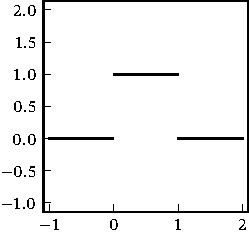
\includegraphics{figures/haar_scaling}
    \caption{Haarのスケーリング関数.}
  \end{minipage}%
  \begin{minipage}{0.5\linewidth}
    \centering
    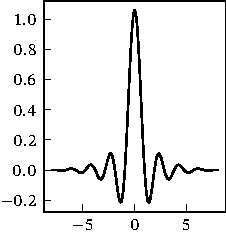
\includegraphics{figures/meyer_scaling}
    \caption{Meyerのスケーリング関数.}
  \end{minipage}
\end{figure}

\section*{演習問題}
\addcontentsline{toc}{section}{演習問題}

\end{document}
